\documentclass[13pt]{article}

\title{Problem 15: Lattice Paths}
\date{2022-06-16}
\author{Rushil Surti}

% \usepackage{amsmath}
\usepackage{tikz}

\begin{document}

\maketitle

\section{Description}

Let R(N) denote the amount of routes that can be taken in a NxN grid from start to finish if you can only move in the right and downward direction.

\section{Task}

Find R(20).

\section{Examples}

R(2) = 6. This is shown in the graphic by:

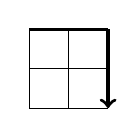
\begin{tikzpicture}
	\draw[step=0.5cm,black,thin] (0, 0) grid (1, 1);
	\draw[very thick] (0, 1) -- (1, 1);
	\draw[very thick, ->] (1, 1) -- (1, 0);
\end{tikzpicture}
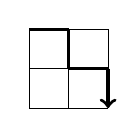
\begin{tikzpicture}
	\draw[step=0.5cm,black,thin] (0, 0) grid (1, 1);
	\draw[very thick] (0, 1) -- (0.5, 1);
	\draw[very thick] (0.5, 1) -- (0.5, 0.5);
	\draw[very thick] (0.5, 0.5) -- (1, 0.5);
	\draw[very thick, ->] (1, 0.5) -- (1, 0);
\end{tikzpicture}
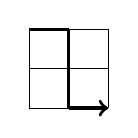
\begin{tikzpicture}
	\draw[step=0.5cm,black,thin] (0, 0) grid (1, 1);
	\draw[very thick] (0, 1) -- (0.5, 1);
	\draw[very thick] (0.5, 1) -- (0.5, 0);
	\draw[very thick, ->] (0.5, 0) -- (1, 0);
\end{tikzpicture}

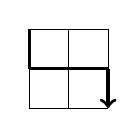
\begin{tikzpicture}
	\draw[step=0.5cm,black,thin] (0, 0) grid (1, 1);
	\draw[very thick] (0, 1) -- (0, 0.5);
	\draw[very thick] (0, 0.5) -- (1, 0.5);
	\draw[very thick, ->] (1, 0.5) -- (1, 0);
\end{tikzpicture}
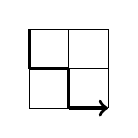
\begin{tikzpicture}
	\draw[step=0.5cm,black,thin] (0, 0) grid (1, 1);
	\draw[very thick] (0, 1) -- (0, 0.5);
	\draw[very thick] (0, 0.5) -- (0.5, 0.5);
	\draw[very thick] (0.5, 0.5) -- (0.5, 0);
	\draw[very thick, ->] (0.5, 0) -- (1, 0);
\end{tikzpicture}
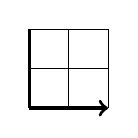
\begin{tikzpicture}
	\draw[step=0.5cm,black,thin] (0, 0) grid (1, 1);
	\draw[very thick] (0, 1) -- (0, 0);
	\draw[very thick, ->] (0, 0) -- (1, 0);
\end{tikzpicture}

\section{Observations}

\end{document}
